\let\negmedspace\undefined
\let\negthickspace\undefined
\documentclass[journal]{IEEEtran}
\usepackage[a5paper, margin=10mm, onecolumn]{geometry}
%\usepackage{lmodern} % Ensure lmodern is loaded for pdflatex
\usepackage{tfrupee} % Include tfrupee package

\setlength{\headheight}{1cm} % Set the height of the header box
\setlength{\headsep}{0mm}     % Set the distance between the header box and the top of the text

\usepackage{gvv-book}
\usepackage{gvv}
\usepackage{cite}
\usepackage{amsmath,amssymb,amsfonts,amsthm}
\usepackage{algorithmic}
\usepackage{graphicx}
\usepackage{textcomp}
\usepackage{xcolor}
\usepackage{txfonts}
\usepackage{listings}
\usepackage{enumitem}
\usepackage{mathtools}
\usepackage{gensymb}
\usepackage{comment}
\usepackage[breaklinks=true]{hyperref}
\usepackage{tkz-euclide} 
\usepackage{listings}
% \usepackage{gvv}                                        
\def\inputGnumericTable{}                                 
\usepackage[latin1]{inputenc}                                
\usepackage{color}                                            
\usepackage{array}                                            
\usepackage{longtable}                                       
\usepackage{calc}                                             
\usepackage{multirow}                                         
\usepackage{hhline}                                           
\usepackage{ifthen}                                           
\usepackage{lscape}
\usepackage{multicol}
\begin{document}

\bibliographystyle{IEEEtran}
\vspace{3cm}

\title{10.3.11}
\author{EE25BTECH11012-BEERAM MADHURI}
% \maketitle
% \newpage
% \bigskip
{\let\newpage\relax\maketitle}

\renewcommand{\thefigure}{\theenumi}
\renewcommand{\thetable}{\theenumi}
\setlength{\intextsep}{10pt} % Space between text and floats


\numberwithin{equation}{enumi}
\numberwithin{figure}{enumi}
\renewcommand{\thetable}{\theenumi}

\textbf{Question}:\\
Find the normal at the point $(1,1)$ on the curve
\begin{align}
2y + x^2 = 3
\end{align}
\textbf{Solution:}
\begin{align}
    2y + x^2 = 3\\
    2y + x^2 -3 = 0
\end{align}
Which can be expressed as the conic:
\begin{align}
\vec{x^\top V x} + 2\vec{u^\top x} + f = 0\\
\vec{V} = \begin{pmatrix}1 & 0 \\0 & 0\end{pmatrix}, \vec{u} = \begin{pmatrix}0 \\1\end{pmatrix}, f = -3
\end{align}
let 
\begin{align}
\vec{p} \begin{pmatrix} 1 \\ 1 \end{pmatrix} , \vec{m} \text{ is normal vector }\\
\vec{m}^\top \vec{(Vp + u)} = 0
\end{align}
substitung the value :
\begin{align}
\vec{m}=\begin{pmatrix} m_1 \\ m_2 \end{pmatrix} \\
\vec{Vp}=\begin{pmatrix}1 & 0 \\0 & 0\end{pmatrix}\begin{pmatrix}
    1\\1 \end{pmatrix}\\
    =\begin{pmatrix} 1\\0 \end{pmatrix}\\
\begin{pmatrix} m_1 \\ m_2 \end{pmatrix} \begin{pmatrix} 1+0\\0+1 \end{pmatrix}=0\\
m_1=-m_2\\
\therefore \vec{m}=\begin{pmatrix} -m \\ m \end{pmatrix}
\end{align}
equation of normal is
\begin{align}
    \vec{m}^\top(\vec{x-p})=0\\
    \begin{pmatrix} -1&1\end{pmatrix}\begin{pmatrix}x-1\\y-1   \end{pmatrix}=0\\
        y=x
\end{align}
Hence equation of normal to $2y + x^2 - 3 = 0$ at $(1,1)$ is $y = x$.

\begin{figure}[H]
    \centering
    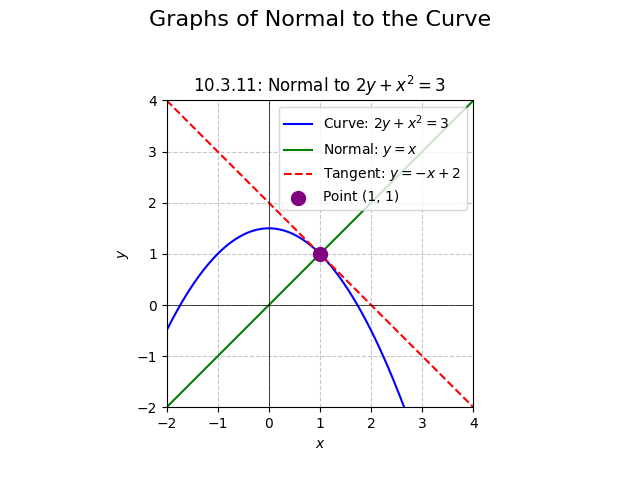
\includegraphics[width=0.85\columnwidth]{figs/graph-17.png}
    \caption{10.3.11}
    \label{fig:placeholder}
\end{figure}
\end{document}
